\section{Methodology}
\label{sec:methodology}


\subsection{Architectural Formulation of \modelname{}}
\label{subsec:architecture}

Let $\mathcal{D} = \{(x_i, y_i)\}_{i=1}^M$ denote a tabular dataset with $M$ samples, where each input vector $x_i = [x_{i1}, x_{i2}, \dots, x_{iN}]^\top \in \R^N$ contains $N$ features, and $y_i \in \{1, 2, \dots, C\}$ represents the target class label across $C$ discrete categories. 

\modelname{} is a three-layer feedforward architecture with interpretable internal states,
shown in Figures~\ref{fig:arch_forward}--\ref{fig:arch_scorecard} together with the
activation function and the scorecard entries it produces:
\begin{enumerate}
    \item A bias-free linear feature projection layer,
    \item A localized triangular activation layer with learnable centers and widths,
    \item A linear output scoring layer producing class logits.
\end{enumerate}

\begin{figure*}[t]
\centering
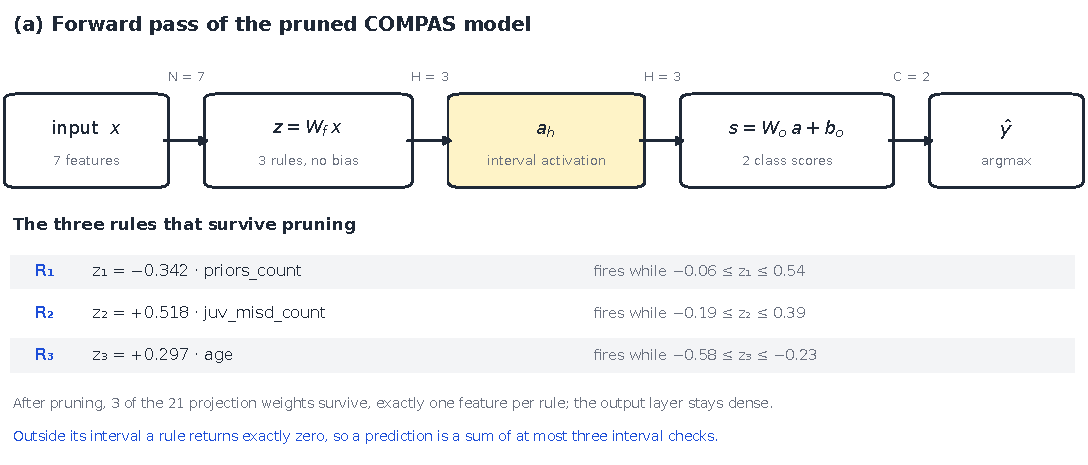
\includegraphics[width=\textwidth]{figures/fig_arch_forward.pdf}
\caption{The \modelname{} forward pass for the protected-attribute-free COMPAS
variant of Section~\ref{subsec:comparative_results}, drawn from its released Compact
checkpoint. A bias-free projection $W_f \in \R^{3 \times 7}$ maps the $N=7$ inputs to
$H=3$ scalars $z_h$; each scalar is passed through a localized activation $a_h$; a
linear output layer maps the three activations to $C=2$ class scores, and the larger
score gives the prediction. The table lists the three rules that survive pruning,
with the weight and firing interval read from the checkpoint.}
\label{fig:arch_forward}
\end{figure*}

\begin{figure*}[t]
\centering
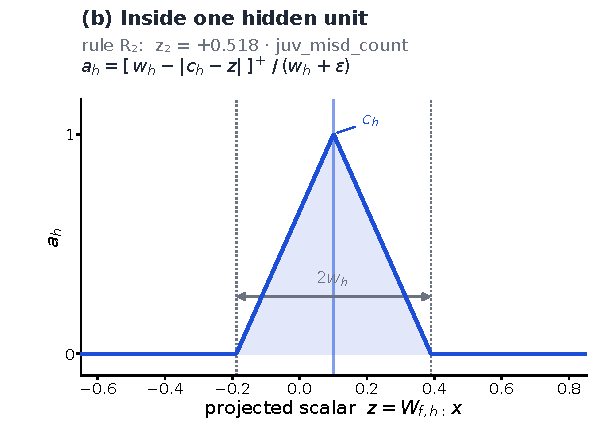
\includegraphics[width=0.55\textwidth]{figures/fig_arch_unit.pdf}
\caption{The activation of a single hidden unit as a function of the projected scalar
$z=W_{f,h:}x$. It peaks at $c_h$, decreases linearly, and is exactly zero for
$|c_h - z| \ge w_h$, so the unit is active only on an interval of width $2w_h$. The
plotted parameters belong to rule $R_2$ of the same Compact model
(the protected-attribute-free COMPAS variant).}
\label{fig:arch_unit}
\end{figure*}

\begin{figure*}[t]
\centering
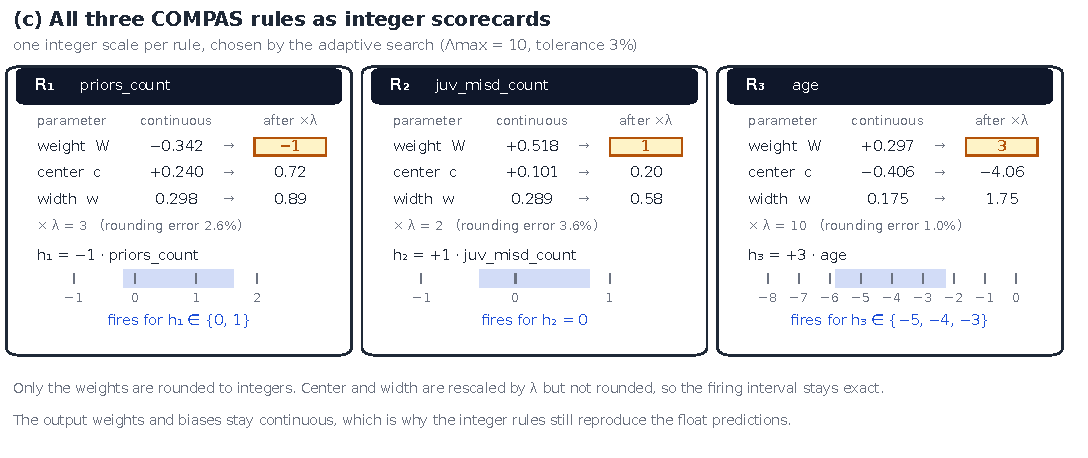
\includegraphics[width=\textwidth]{figures/fig_arch_scorecard.pdf}
\caption{Rule-level integer quantization applied to all three rules of the same
COMPAS Compact model. Each rule
uses its own scale $\lambda_h$, chosen by the adaptive search of
Section~\ref{subsec:scorecard} (the budget is printed in the panel): the continuous
weight $W$ is multiplied by $\lambda_h$ and rounded to the small integer in the shaded
box, while the center $c$ and width $w$ are rescaled by the same $\lambda_h$ but not
rounded, so the firing interval stays exact. Each card shows the integer point sum
$h_h$ and the integer values it must take for the rule to fire. The output layer $W_o$
and the bias $b_o$ remain continuous.}
\label{fig:arch_scorecard}
\end{figure*}

\subsubsection{Layer 1: Bias-Free Linear Projection}
Given an input sample $x \in \R^N$, the model first computes $H$ linear combinations using a weight matrix $W_f \in \R^{H \times N}$:
\begin{equation}
\label{eq:linear_projection}
h = W_f x, \quad \text{where } h_h = \sum_{j=1}^N W_{f,hj} x_j, \quad \forall h \in \{1, \dots, H\}.
\end{equation}
In this equation, each row $W_{f,h:} \in \R^N$ acts as a feature projection vector for the $h$-th hidden neuron. 

We omit a bias term in this layer ($bias = \text{False}$). As a result, when the input is zero ($x = 0$), the projection is also zero ($h = 0$). As we show in Section~\ref{subsec:bias_shifting}, this choice matters: when a rule's input connections are pruned to zero, its baseline behavior becomes a constant that does not depend on the input, and it can be absorbed exactly into the output bias.


\subsubsection{Layer 2: Localized Triangular Rule Activation}
Standard neural networks typically use monotonic activations such as ReLU ($\max(0, z)$), which stay active over unbounded regions of the input space. In contrast, \modelname{} equips each hidden unit $h$ with two learnable scalar parameters: a center $c_h \in \R$ and an unconstrained base width parameter $\tilde{w}_h \in \R$. We define the operational half-width $w_h$ as the magnitude of the base width,
\begin{equation}
w_h = |\tilde{w}_h|,
\end{equation}
so that the effective bandwidth is strictly positive whenever $\tilde{w}_h \neq 0$.

The localized triangular activation $\text{Act}_h(x)$ is defined as:
\begin{equation}
\label{eq:triangular_activation}
a_h(x) = \text{Act}_h(x) = \frac{\max\Big(0, \, w_h - |c_h - h_h|\Big)}{w_h + \epsilon},
\end{equation}
where $\epsilon = 10^{-8}$ is a small constant added to the denominator to avoid division by zero when the base width collapses to zero; it does not change the support of the rule.

The activation has three useful properties (Figure~\ref{fig:arch_unit}):
\begin{itemize}
    \item \textbf{Bounded Output Range:} $a_h(x) \in [0, 1]$ for all $x \in \R^N$.
    \item \textbf{Centroid Peak:} When the projection exactly matches the center ($h_h = c_h$), the activation reaches its maximum value $a_h(x) = w_h/(w_h+\epsilon)$, which equals $1$ up to the $10^{-8}$ denominator regularizer.
    \item \textbf{Compact Support (Hard Zero Region):} When the distance between the projection and the center is at least the width ($|c_h - h_h| \ge w_h$), the activation is identically zero ($a_h(x) = 0.0$).
\end{itemize}

During training, an optional dropout mask with probability $p_{drop}$ is applied to the activation vector $a(x) = [a_1(x), \dots, a_H(x)]^\top$ to prevent co-adaptation among redundant rules.

\subsubsection{Layer 3: Class-Specific Logit Scoring}
The activation vector $a(x) \in \R^H$ is fed into a linear classification layer parameterized by a weight matrix $W_o \in \R^{C \times H}$ and a class bias vector $b_o \in \R^C$. The unnormalized class score (logit) for class $c \in \{1, \dots, C\}$ is computed as:
\begin{equation}
\label{eq:output_scoring}
s_c(x) = b_{o,c} + \sum_{h=1}^H W_{o,ch} \, a_h(x).
\end{equation}

The output layer is trained without a bias parameter, so the logits depend only on the
rule activations. As shown in Section~\ref{subsec:bias_shifting}, the bias vector $b_o$
is created during post-training compaction, when the constant baseline activations of
pruned rules are absorbed into it.

The coefficient $W_{o,ch}$ is the signed vote that rule $h$ casts for class $c$. A positive value adds evidence for class $c$ when the rule fires; a negative value counts against class $c$.

The final predicted class label $\hat{y}$ is obtained via the argmax operator:
\begin{equation}
\hat{y} = \arg\max_{c \in \{1, \dots, C\}} s_c(x).
\end{equation}

The softmax transformation converts the class logits into normalized class probability estimates:
\begin{equation}
P(Y = c \mid x) = \frac{\exp(s_c(x))}{\sum_{k=1}^C \exp(s_k(x))}.
\end{equation}


\subsection{Geometric Characterization: Localized Convex Slabs}
\label{subsec:geometry}

To understand what a hidden unit represents, we characterize the region in the input space $\R^N$ on which it is active.

\begin{definition}[Localized Convex Slab Rule]
For any hidden unit $h \in \{1, \dots, H\}$ with projection vector $W_{f,h:} \in \R^N$, center $c_h$, and width $w_h > 0$, the activation is strictly positive on the open slab $c_h - w_h < \sum_j W_{f,hj} x_j < c_h + w_h$ and exactly zero elsewhere. Its \emph{closed support}---the closure of that set, i.e.\ the inputs on which the rule fires or reaches its boundary---is the convex slab
\begin{equation}
\label{eq:convex_slab}
\mathcal{S}_h = \left\{ x \in \R^N : c_h - w_h \le \sum_{j=1}^N W_{f,hj} x_j \le c_h + w_h \right\}.
\end{equation}
\end{definition}


In classical rule systems such as decision tree leaves, a rule is an axis-aligned
hyperrectangle $\bigwedge_j (l_j \le x_j \le u_j)$. Unless $W_{f,h:}$ has a single
non-zero entry, $\mathcal{S}_h$ is instead a \textbf{convex slab}: the closed
region between two parallel hyperplanes orthogonal to $W_{f,h:}$. When pruning
leaves one active feature, the slab becomes a 1D interval, $x_j$ lying between
$(c_h-w_h)/W_{f,hj}$ and $(c_h+w_h)/W_{f,hj}$ (swapped when $W_{f,hj}<0$); with
two features it is an oblique strip. \modelname{} therefore generalizes
axis-aligned interval rules to oblique ones while retaining sharp geometric
boundaries.


\subsubsection{Piecewise Linearity and Breakpoints}
Along the one-dimensional projected coordinate $z = W_{f,h:} x$, the activation function $a_h(z)$ is continuous and piecewise linear, with exactly three derivative breakpoints:
\begin{equation}
z \in \{ c_h - w_h, \; c_h, \; c_h + w_h \}.
\end{equation}
The derivative of the activation with respect to the projected input $z$ is:
\begin{equation}
\frac{\partial a_h}{\partial z} = 
\begin{cases}
+1 / (w_h + \epsilon), & \text{if } c_h - w_h < z < c_h, \\
-1 / (w_h + \epsilon), & \text{if } c_h < z < c_h + w_h, \\
0, & \text{if } z < c_h - w_h \text{ or } z > c_h + w_h.
\end{cases}
\end{equation}
This piecewise-linear structure ensures that the entire network maps the input space into hyperplane-bounded response regions, which makes exact sensitivity analysis and boundary verification straightforward.


\subsection{Training Protocol and Structural Sparsification}
\label{subsec:pruning}

To obtain a compact and human-auditable rule set, we train \modelname{} through a two-stage process: regularized optimization followed by Iterative Magnitude Pruning (IMP).

\subsubsection{Regularized Loss Function}
We train the network end-to-end using standard gradient descent. The total training objective combines the cross-entropy classification loss with dual $\ell_1$ regularization penalties~\cite{tibshirani1996lasso} on both weight layers:
\begin{equation}
\label{eq:total_loss}
\mathcal{L}(\theta) = \mathcal{L}_{CE}(y, s(x)) + \lambda_1 \|W_f\|_1 + \lambda_2 \|W_o\|_1,
\end{equation}
where $\mathcal{L}_{CE}$ is the standard multiclass cross-entropy:
\begin{equation}
\mathcal{L}_{CE} = - \frac{1}{M} \sum_{i=1}^M \sum_{c=1}^C \mathbb{I}(y_i = c) \log \left( \frac{\exp(s_c(x_i))}{\sum_{k=1}^C \exp(s_k(x_i))} \right).
\end{equation}
The $\ell_1$ penalty on $W_f$ encourages sparsity in feature connections, driving redundant feature weights to zero and reducing the number of variables in each rule. The $\ell_1$ penalty on $W_o$ encourages the network to use only a minimal subset of rules for class scoring.

\subsubsection{Iterative Magnitude Pruning (IMP)}
While $\ell_1$ regularization shrinks weights, gradient descent alone rarely sets parameters to exact zeros. To produce sparse, inspectable sub-networks, we apply Iterative Magnitude Pruning (IMP)~\cite{frankle2018lottery,han2015learning} to the projection matrix $W_f$:
\begin{enumerate}
    \item \textbf{Dense Training:} Train the initial model with $H$ hidden units until convergence on the training set using validation accuracy for early stopping.
    \item \textbf{Magnitude Masking:} Identify the bottom $p\%$ (e.g., $p = 20\%$) of non-zero entries in $|W_f|$ across the layer and set their binary mask entries to zero.
    \item \textbf{Fine-Tuning:} Fine-tune the remaining unmasked parameters for several epochs to allow the network to recover predictive performance.
    \item \textbf{Iteration:} Repeat steps 2 and 3 iteratively until the desired sparsity target or validation performance threshold is reached.
\end{enumerate}

Because step 2 removes a fixed fraction of the \emph{remaining} weights, the surviving connections follow a geometric schedule. In the continuous limit
\begin{equation}
\label{eq:link_budget}
L = H_0 N \,(1-p)^{K},
\end{equation}
while the implemented recurrence rounds at every step, $R_{k+1} = R_k - \mathrm{round}(p R_k)$ with $R_0 = H_0N$. For the registered configurations this gives $416 \rightarrow 6$ on COMPAS and $3{,}072 \rightarrow 135$ on German Credit, so the closed form is accurate to about one unit. Pruned entries stay exactly zero during fine-tuning, because the mask is applied on every forward pass; the schedule is therefore an upper bound rather than a target training may overshoot.

The realized count can still fall below it. The two-tier filter of Section~\ref{subsec:two_tier} removes rules that never fire on the training partition, and such a rule takes its connections with it: the German Credit Compact checkpoint holds $135$ connections after pruning and $124$ after six dead rules are removed. Section~\ref{subsec:stability} reports the ranges.

Three quantities are easy to conflate: \emph{connections} (surviving entries of
$W_f$, i.e.\ (rule, feature) pairs), \emph{rules} (non-empty rows, $H^*$), and
\emph{features} (columns used by at least one rule). Because one feature may serve
several rules, connections $\ge$ features and neither fixes the other. The
schedule in Equation~\eqref{eq:link_budget} controls the connection budget, not
how many \emph{distinct} features the surviving rules touch, so we report all
three counts.

\subsubsection{Two-Tier Rule Filtering: Structural and Empirical}
\label{subsec:two_tier}
After the pruning iterations, the model may still contain weights of negligible magnitude (e.g., $10^{-5}$) or rules that never fire on the data. We use a two-tier filtering procedure to identify such inactive rules:
\begin{itemize}
    \item \textbf{Tier 1 (Structurally Empty Rules):} A rule $h$ is structurally empty if the sum of its absolute input weights is below a small threshold $\tau_w$ (e.g., $\tau_w = 10^{-4}$):
    \begin{equation}
    \sum_{j=1}^N |W_{f,hj}| \le \tau_w \implies h \in \mathcal{H}_{struct}.
    \end{equation}
    Such rules have effectively lost all connections to the input features.
    \item \textbf{Tier 2 (Empirically Dead Rules):} A rule $h$ is empirically dead if its maximum activation over the training data $\mathcal{D}_{\text{train}}$ falls below an activation threshold $\tau_a$ (e.g., $\tau_a = 10^{-4}$), or if its empirical sample coverage is lower than a threshold $\tau_{cov}$
($\tau_{cov} = 0$ in all reported runs, so in practice the activation criterion alone
decides):
    \begin{align}
    &\max_{x \in \mathcal{D}_{\text{train}}} a_h(x) \le \tau_a \nonumber\\
    &\text{or}\quad \frac{1}{|\mathcal{D}_{\text{train}}|} \sum_{x \in \mathcal{D}_{\text{train}}} \mathbb{I}(a_h(x) > \tau_a) \le \tau_{cov}.
    \end{align}
    Such rules are inactive on the training data. Unlike Tier~1, this criterion is
    empirical: a rule that is inactive on the training partition may still fire on
    a held-out point, so removing it is not covered by
    Proposition~\ref{prop:bias_shifting} and can introduce a small drift. We
    therefore treat Tier~2 as a model-selection step and report the resulting
    held-out accuracy and fidelity rather than assuming exactness. In our
    experiments it removes $18$ rules from the Synthetic Global Best model and
    $6$ from German Credit Compact, and none from the other eight
    checkpoint/dataset combinations; all reported accuracies and fidelities are
    measured after these removals.
\end{itemize}

\subsubsection{Exact Bias Shifting for Pruned Rules}
\label{subsec:bias_shifting}

When a structurally empty rule $h \in \mathcal{H}_{struct}$ is found, removing it directly can change the network's output logits. This happens because if its center and width satisfy $|c_h| < w_h$, the unit produces a non-zero baseline activation when its input projection is zero ($h_h = 0$). 

Here we prove that this constant baseline can be shifted into the output bias with no change to the model's predictions.

\begin{proposition}[Exact Bias Shifting for Pruned Rules]
\label{prop:bias_shifting}
Let $h \in \mathcal{H}_{struct}$ be a structurally empty rule unit such that $W_{f,h:} = 0$. For any input $x \in \R^N$, the hidden projection is identically zero ($h_h = W_{f,h:} x = 0$), and the unit's activation is an invariant constant:
\begin{equation}
\label{eq:baseline_activation}
a_h^{(0)} = \frac{\max\Big(0, \, w_h - |c_h|\Big)}{w_h + \epsilon}.
\end{equation}
If rule $h$ is removed from the network and the output bias vector $b_o \in \R^C$ is updated to:
\begin{equation}
\label{eq:bias_update}
b_o^{\text{new}} = b_o^{\text{old}} + W_{o,:,h} \cdot a_h^{(0)},
\end{equation}
then the input-output mapping of the compressed model is identical to that of the uncompressed model for all inputs $x \in \R^N$:
\begin{equation}
s_c^{\text{new}}(x) \equiv s_c^{\text{old}}(x), \quad \forall c \in \{1, \dots, C\}, \; \forall x \in \R^N.
\end{equation}
As a result, removing the rule causes no change in the logits ($\Delta \text{Logit}(x) \equiv 0$).
\end{proposition}

\begin{proof}
Consider the logit score for class $c$ in the original network before removing rule $h$:
\begin{equation}
s_c^{\text{old}}(x) = b_{o,c}^{\text{old}} + \sum_{k \ne h} W_{o,ck} \, a_k(x) + W_{o,ch} \, a_h(x).
\end{equation}
Because $W_{f,h:} = 0$, the projected scalar is $h_h = \sum_{j=1}^N 0 \cdot x_j = 0$ for every $x \in \R^N$. Substituting $h_h = 0$ into the triangular activation function (Equation~\ref{eq:triangular_activation}) gives:
\begin{align}
a_h(x) &= \frac{\max\Big(0, \, w_h - |c_h - 0|\Big)}{w_h + \epsilon} \nonumber \\
&= \frac{\max\Big(0, \, w_h - |c_h|\Big)}{w_h + \epsilon} = a_h^{(0)}.
\end{align}
Notice that $a_h^{(0)}$ is independent of $x$. Thus, the contribution of rule $h$ to class $c$ is the constant value $W_{o,ch} \, a_h^{(0)}$. We can rewrite the score as:
\begin{align}
s_c^{\text{old}}(x) &= \left( b_{o,c}^{\text{old}} + W_{o,ch} \, a_h^{(0)} \right) + \sum_{k \ne h} W_{o,ck} \, a_k(x) \\
&= b_{o,c}^{\text{new}} + \sum_{k \ne h} W_{o,ck} \, a_k(x) \\
&= s_c^{\text{new}}(x).
\end{align}
This holds identically for all classes $c \in \{1, \dots, C\}$ and all inputs $x \in \R^N$, which completes the proof.
\end{proof}

When multiple hidden units $\mathcal{H}_{struct} = \{h_1, h_2, \dots, h_K\}$ are structurally pruned simultaneously, their baseline contributions sum linearly:
\begin{equation}
b_o^{\text{new}} = b_o^{\text{old}} + \sum_{h \in \mathcal{H}_{struct}} W_{o,:,h} \cdot a_h^{(0)}.
\end{equation}
This allows the network to be safely compacted from $H$ units to $H - |\mathcal{H}_{struct}|$ units in a single operation, guaranteeing zero prediction drift.



\subsection{Rule-Level Integer Quantization and Scorecard Representation}
\label{subsec:scorecard}

In clinical medicine and credit underwriting, domain practitioners favor scorecard models because individual rules can be audited using simple integer arithmetic~\cite{gage2001validation,hlongwane2024transparency,ustun2016supersparse}.

Instead of quantizing the whole multi-class network into a single global integer, \modelname{} uses \emph{rule-level integer quantization}. This maps each rule's continuous projection weights $W_f$ to small integers, while the linear output layer stays continuous and transparent.

\subsubsection{Per-Rule Adaptive Integer Scaling}
For each surviving rule $h \in \{1, \dots, H\}$, the input projection parameters are continuous floats: $W_{f,h:} \in \R^N$, center $c_h \in \R$, and width $w_h \in \R^+$. We seek an optimal positive integer scale factor $\lambda_h \in \{1, 2, \dots, \Lambda_{\max}\}$ that converts continuous projection weights into low-magnitude integers while minimizing rounding distortion.

For any candidate multiplier $\lambda \in \{1, \dots, \Lambda_{\max}\}$, the rounded integer feature weights are defined as:
\begin{equation}
\widetilde{W}_{f,hj}(\lambda) = \text{round}(\lambda \, W_{f,hj}) \in \mathbb{Z}.
\end{equation}
Let $\mathcal{F}_h = \{j : |W_{f,hj}| > \tau_w\}$ denote the set of active features in rule $h$. The relative parameter rounding error at scale $\lambda$ is computed as:
\begin{equation}
\mathcal{E}_h(\lambda) = \frac{\sum_{j \in \mathcal{F}_h} |\lambda W_{f,hj} - \widetilde{W}_{f,hj}(\lambda)|}{\sum_{j \in \mathcal{F}_h} |\lambda W_{f,hj}| + \epsilon}.
\end{equation}

To avoid unnecessarily large integer coefficients that would impair human readability, we select the smallest scale $\lambda_h^*$ that achieves an acceptable rounding tolerance $\tau_{tol}$ (1--6\% in our experiments, depending on the dataset):
\begin{equation}
\label{eq:adaptive_scale}
\lambda_h^* = \min \left\{ \lambda \in \{1, \dots, \Lambda_{\max}\} : \mathcal{E}_h(\lambda) \le \tau_{tol} \right\}.
\end{equation}
If no integer satisfies the threshold, we choose the scale that minimizes $\mathcal{E}_h(\lambda)$ across the search grid. The pair $(\Lambda_{\max}, \tau_{tol})$ is fixed once per dataset and model variant and is not adapted per rule instance; it is part of the reported operating point rather than a per-example choice. Section~\ref{subsec:quantization_fidelity} reports the resulting fidelity and integer spans, and Section~\ref{subsec:limitations} notes how these budgets were set.

\subsubsection{Scorecard Rule Formulation}
With the selected scale $\lambda_h^*$, each hidden neuron becomes an explicit \emph{integer scorecard rule}:
\begin{enumerate}
    \item \textbf{Integer Rule Score:} The stakeholder computes a discrete point sum using only integer coefficients:
    \begin{equation}
    \tilde{h}_h(x) = \sum_{j \in \mathcal{F}_h} \widetilde{W}_{f,hj} \, x_j.
    \end{equation}
    On tabular benchmarks, the resulting integer weights $\widetilde{W}_{f,hj}$ span only a few integer values on binary tasks (e.g., $[-3, 3]$ on COMPAS and $[-5, 6]$ for the German Credit Compact model), and a wider range on the 20-class task.
    \item \textbf{Activation Interval Verification:} The rule's effective center and width are scaled consistently: $\widetilde{c}_h = \lambda_h^* c_h$ and $\widetilde{w}_h = \lambda_h^* w_h$. The rule activation condition is verified against these bounds:
    \begin{equation}
    \widetilde{c}_h - \widetilde{w}_h \le \tilde{h}_h(x) \le \widetilde{c}_h + \widetilde{w}_h.
    \end{equation}
    If the integer score falls within this interval, the rule fires with intensity:
    \begin{equation}
    \tilde{a}_h(x) = \frac{\widetilde{w}_h - |\widetilde{c}_h - \tilde{h}_h(x)|}{\widetilde{w}_h} \in [0, 1].
    \end{equation}
    Otherwise, $\tilde{a}_h(x) = 0$.
\end{enumerate}

\subsubsection{Interpreting Integer Weights and Raw Feature Scales}
\label{subsubsec:standardized_vs_raw}

Because tabular datasets mix units---loan amounts, durations, binary indicators---
continuous features are standardized to zero mean and unit variance prior to
training:
\begin{equation}
\tilde{x}_j = \frac{x_j^{\text{raw}} - \mu_j}{\sigma_j}.
\label{eq:standardization}
\end{equation}
Standardization stabilizes gradient optimization and ensures that the $\ell_1$
penalty treats all features fairly. Below, $x$ denotes the standardized vector and
$x^{\text{raw}}$ the same instance in native units. The same integer rule can then
be read in two coordinate systems.
\begin{enumerate}
    \item \textbf{Standardized sensitivity (relative point tally):} since every
    standardized feature has $\sigma = 1$, each integer weight reflects the effect
    of a one-standard-deviation change. Weights of $+2$ on credit amount and $-1$
    on duration mean that a one-standard-deviation increase in credit amount adds
    twice as much evidence toward firing as a one-standard-deviation increase in
    duration subtracts. This avoids comparing incompatible physical units.

    \item \textbf{Exact affine de-normalization:} domain experts may prefer the
    original physical units. For rule $h$, define the native-coordinate score
    \begin{equation}
    S_h(x^{\text{raw}})
    =
    \sum_{j \in \mathcal{F}_h}
    \left(\frac{\widetilde{W}_{f,hj}}{\sigma_j}\right)x_j^{\text{raw}}.
    \label{eq:raw_score}
    \end{equation}
    Substituting $\tilde{x}_j=(x_j^{\text{raw}}-\mu_j)/\sigma_j$ into
    $\tilde{h}_h$ gives
    \begin{equation}
    \tilde{h}_h(x)
    =
    S_h(x^{\text{raw}})-\Delta c_h,
    \qquad
    \Delta c_h
    =
    \sum_{j \in \mathcal{F}_h}
    \widetilde{W}_{f,hj}\frac{\mu_j}{\sigma_j}.
    \label{eq:center_shift}
    \end{equation}
    Adding $\Delta c_h$ to the firing condition
    $\widetilde{c}_h-\widetilde{w}_h\le\tilde{h}_h(x)\le\widetilde{c}_h+\widetilde{w}_h$
    yields
    \begin{equation}
    \label{eq:physical_bounds}
    \widetilde{c}_h+\Delta c_h-\widetilde{w}_h
    \le S_h(x^{\text{raw}})
    \le \widetilde{c}_h+\Delta c_h+\widetilde{w}_h.
    \end{equation}
    The sign flips because the $-\Delta c_h$ in \eqref{eq:center_shift} becomes
    $+\Delta c_h$ in the center of \eqref{eq:physical_bounds}. For a univariate
    rule this is an interval in the original feature; for a multivariate rule it is
    the same oblique slab in native units.
\end{enumerate}

\noindent\textit{What is exact?} Equation~\eqref{eq:physical_bounds} is an exact
change of coordinates for the \emph{quantized} rule and adds no approximation
error. It does not undo the rounding of $W_{f,hj}$; agreement with the float model
is the empirical fidelity reported in
Section~\ref{subsec:quantization_fidelity}. This dual representation lets
practitioners score with small integers while retaining the exact physical
boundaries of the quantized rule for audit.

\subsubsection{Continuous Output Scoring and Quantization Fidelity}
Once the rule activations $\tilde{a}_h(x)$ are computed, the class logits follow
from the output layer:
\begin{equation}
s_c^{(quant)}(x) = b_{o,c} + \sum_{h=1}^H W_{o,ch} \, \tilde{a}_h(x),
\end{equation}
where $W_{o,ch}$ and $b_{o,c}$ are transparent continuous voting weights. Two
fidelity metrics are measured on the test partition:
\begin{itemize}
    \item \textbf{Prediction agreement (fidelity):} the proportion of test
    instances on which the quantized and float models agree:
    \begin{equation}
    \label{eq:fidelity}
    \text{Fidelity} = \frac{1}{M_{test}} \sum_{i=1}^{M_{test}} \mathbb{I}\left(\hat{y}_i^{(quant)} = \hat{y}_i^{(float)}\right) \times 100\%.
    \end{equation}
    \item \textbf{Accuracy change:}
    $\Delta \text{Acc} = \text{Acc}^{(quant)} - \text{Acc}^{(float)}$.
\end{itemize}

\subsection{Analytical Interpretability Toolkit}
\label{subsec:analytical_xai}

Unlike black-box models that need sampling-based surrogates such as SHAP or LIME,
\modelname{} computes its explanations in closed form from the learned parameters.

\subsubsection{Local Decision Decomposition}
For a query $x$, the active rule set is $\mathcal{A}(x) = \{ h : a_h(x) > 0 \}$, and
\begin{equation}
s_c(x) = b_{o,c} + \sum_{h \in \mathcal{A}(x)} \text{Cont}_{h,c}(x),
\end{equation}
where $\text{Cont}_{h,c}(x) = W_{o,ch} \, a_h(x)$.
The baseline term $b_{o,c}$ collects the constant contributions of rules removed
during compaction, and each active rule contributes an exact number of points.
This is an algebraic identity, so it has zero surrogate error.

\subsubsection{Global Feature Influence}
Global influence combines the within-rule weight $|W_{f,hj}|$, the downstream
voting power $\|W_{o,:,h}\|_1$, and the empirical activation coverage
\begin{equation}
\text{Coverage}_h = \frac{1}{|\mathcal{D}_{\text{train}}|} \sum_{x \in \mathcal{D}_{\text{train}}} a_h(x),
\end{equation}
as
\begin{equation}
\label{eq:feature_influence}
I_j = \sum_{h=1}^H |W_{f,hj}| \cdot \|W_{o,:,h}\|_1 \cdot \text{Coverage}_h,
\end{equation}
normalized to $I_j^{\%} = 100\,I_j / \sum_k I_k$. The coverage term keeps rules
with large weights but negligible firing from inflating a feature's score. $I_j$
is a model-derived attribution, not a causal effect or a Shapley value.

\subsubsection{Exact Partial Response Curves}
Because the model is piecewise linear, the marginal response to one feature
follows analytically, with no grid and no simulation. Let $x_j$ vary over
$[f_{\min, j}, f_{\max, j}]$ with the other features fixed. For each rule with
$W_{f,hj} \ne 0$ the projected scalar is affine,
\begin{equation}
h_h(x_j) = W_{f,hj} \, x_j + b_h^{(j)}, \quad b_h^{(j)} = \sum_{k \ne j} W_{f,hk} \, x_k,
\end{equation}
and the activation changes slope only at three breakpoints, named by their slab
edge in the projected coordinate $z = h_h$:
\begin{align}
\label{eq:breakpoints}
v_{h}^{-} &= \frac{c_h - w_h - b_h^{(j)}}{W_{f,hj}}, \quad
v_{h}^{0} = \frac{c_h - b_h^{(j)}}{W_{f,hj}}, \nonumber \\
v_{h}^{+} &= \frac{c_h + w_h - b_h^{(j)}}{W_{f,hj}}.
\end{align}
Dividing by $W_{f,hj}$ reverses the inequality when the coefficient is negative, so
$v_h^{-}$ may exceed $v_h^{+}$; the ordering is imposed by sorting, not by the
labels. The sorted set
\begin{equation}
\mathcal{V}_j = \text{sort}\left( \bigcup_{h : W_{f,hj} \ne 0} \{ v_h^{-}, v_h^{0}, v_h^{+} \} \cap [f_{\min, j}, f_{\max, j}] \right)
\end{equation}
partitions the domain into intervals $[v_k, v_{k+1}]$ on which the logit response
is strictly affine. Evaluating the network once per breakpoint therefore gives the
exact curve, with a number of forward passes proportional to the rule count.

\subsubsection{Closed-Form Recourse}
Actionable recourse asks for the smallest feature change that overturns an
unfavorable decision. Black-box counterfactuals rely on gradient or heuristic
search; \modelname{} solves the piecewise-linear equation directly. For an
instance assigned class $c_{\text{orig}} = \arg\max_k s_k(x)$ and a target
$c_{\text{target}}$, the margin along feature $j$ is
\begin{equation}
\Delta s_j(x_j) = s_{c_{\text{target}}}(x_{-j}, x_j) - s_{c_{\text{orig}}}(x_{-j}, x_j),
\end{equation}
which is affine on each breakpoint interval. Wherever the margin changes sign, the
crossing follows in closed form:
\begin{equation}
\label{eq:exact_recourse}
v_j^* = v_k - \Delta s_j(v_k) \cdot \frac{v_{k+1} - v_k}{\Delta s_j(v_{k+1}) - \Delta s_j(v_k)}.
\end{equation}
If a feature crosses more than once, \modelname{} keeps the root minimizing
$|\Delta x_j| = |v_j^* - x_j^{(0)}|$ and ranks features by the same effort. Because
the root sits on the decision boundary, the returned value is advanced by at most
$10^{-3}$ of the interval width toward the target side and the margin sign is
verified there. The search can be restricted to mutable attributes; the zero
crossing is a geometric candidate, and deployment still requires domain-specific
causal and feasibility checks.

\subsubsection{Architectural Feature Co-occurrence}
Co-occurrence is read directly from the pruned topology. With the incidence
matrix $\text{Mask}_{f,hj} = \mathbb{I}(|W_{f,hj}| > \tau_w)$, the count matrix is
$C = \text{Mask}_f^\top \text{Mask}_f$, and the pairwise Jaccard index is
\begin{equation}
\label{eq:jaccard}
J_{jk} = \frac{C_{jk}}{C_{jj} + C_{kk} - C_{jk}} \in [0, 1].
\end{equation}
High $J_{jk}$ marks features the network treats as an inseparable pair; the
measure is structural, not a causal interaction test.
